% ===================================================================
\chapter{Discussion}
\label{ch:discussion}

This chapter weighs the two algorithms against each other for the application
that motivates the thesis, considers how the results scale and what the
compression ratio really measures, compares the hardware and the results with
the baseline, and sets out the limits of what the evidence supports.

\section{Which algorithm for a sensor front end?}
\label{sec:choice}

On compression ratio, DRHE and LPC are close, and which one leads depends on
the dictionary rather than on the predictors (Section~\ref{sec:dictresult}). On
logic they are level. The decisive differences are elsewhere.

\paragraph{Streaming.} DRHE's output depends only on samples already received,
so it emits compressed data as the raw data arrives, needs no frame buffer, and
its output lags its input by \SI{13}{\micro\second}. LPC's coefficients are sums
over every ramp of the frame, so its first output bit has to wait for its last
input sample: \SI{3.0}{\milli\second} of latency and a \SI{3.0}{\mebi bit}
buffer at this frame size. That is a property of the algorithm, not of this
implementation; no amount of scheduling removes it while the coefficients are
fitted to the frame being compressed.

\paragraph{Memory.} A compressor between the range FFT and the memory bus of a
radar sensor has little memory to spare, and LPC's buffer grows with the frame
(Section~\ref{sec:scaling}). DRHE's state also grows, with the number of range
bins and transmitters, but it is a fraction of a frame.

\paragraph{Where LPC is attractive.} LPC's costs fall on the compressor only.
Its decoder is the cheaper of the two --- no data memory, eight DSP slices ---
because the coefficients arrive ready-made. Where latency of a few milliseconds
is acceptable and the sensor has memory to spare, LPC's \SI{4}{\percent} better
ratio is available. A backward-adaptive LPC, fitting its coefficients to
\emph{previous} frames instead of the current one, would remove both the buffer
and the latency at some cost in ratio, and is a natural next step.

\begin{keybox}
\textbf{Recommendation.} For a streaming sensor-edge compressor, DRHE is the
better choice: it is lossless, compresses by \num{4.2} with a matched
dictionary, keeps up with the data with a wide margin, needs no frame buffer,
and adds microseconds rather than milliseconds of latency. LPC compresses about
\SI{4}{\percent} better, but only by waiting for and storing every frame.
\end{keybox}

\section{Scaling to larger frames}
\label{sec:scaling}

The hardware path compresses four of the cascade's sixteen receive channels,
because four complex 16-bit samples fill the 128-bit stream. The following
estimates scale the measured figures linearly; they are not measurements.

\begin{itemize}
\item \textbf{All 16 receive channels} quadruple the data per frame. DRHE would
take about \SI{2.5}{\milli\second} per frame and LPC about
\SI{13}{\milli\second}, both comfortably within the \SI{200}{\milli\second}
frame period of the ColoRadar capture, but LPC would need a
\SI{12}{\mebi bit} frame buffer and its latency would grow to about
\SI{12}{\milli\second}.
\item \textbf{Kiem's use case} --- 1024 ramps of 1024 samples, four channels,
a \SI{50}{\milli\second} cycle and a \SI{15}{\milli\second} compression budget
--- needs \SI{2.4}{Gbit/s} at the ADC. After the range FFT each frame is
\SI{8.4}{\mega\byte} of complex 16-bit data (512 bins of 16-bit $I$ and $Q$
per ramp and channel), delivered in the \SI{21}{\milli\second} of
acquisition: about \SI{3.2}{Gbit/s} at the compressor's input. DRHE's measured \SI{5.1}{Gbit/s} keeps up without any
buffer. LPC as built would take about \SI{69}{\milli\second} per
frame, longer than the whole cycle, and would need an \SI{8.4}{\mega\byte} frame
buffer against roughly \SI{4.4}{\mega\byte} of block and UltraRAM on this device.
\end{itemize}

\noindent
DRHE scales with the data rate; LPC scales with the frame size, and on large
frames it runs out of both time and memory. Its time per frame could be cut
by about a third by overlapping its passes and amortising the per-bin pipeline
fill (Section~\ref{sec:lpcimpl}), and further only by processing several bins
in parallel, but its buffer and its latency would remain.

\section{What the compression ratio measures}
\label{sec:ratiomeaning}

Figure~\ref{fig:bits} follows one value through the compressor, in bits. The
16-bit container starts with 16. Because the FX16 scale is fixed to a
theoretical full-scale signal and the ColoRadar capture sits far below it, the
largest code over 50 frames is 437, so only $\log_2 437 + 1 = 9.77$ bits ever
carry information; the other 6.2 are copies of the sign bit. Removing them is a
factor of \num{1.64}, and any entropy coder does it whether or not anything is
predicted. The coder then exploits the sparsity of a range-FFT frame --- most
bins hold noise near zero and a few hold targets --- for a further factor of
\num{2.12}, reaching \num{4.60} bits per value. Only then does prediction act,
taking DRHE to \num{4.27} bits (a factor of \num{1.08}), and the re-derived
dictionary takes it to \num{3.79} (\num{1.12}).

\begin{figure}[htbp]
\centering
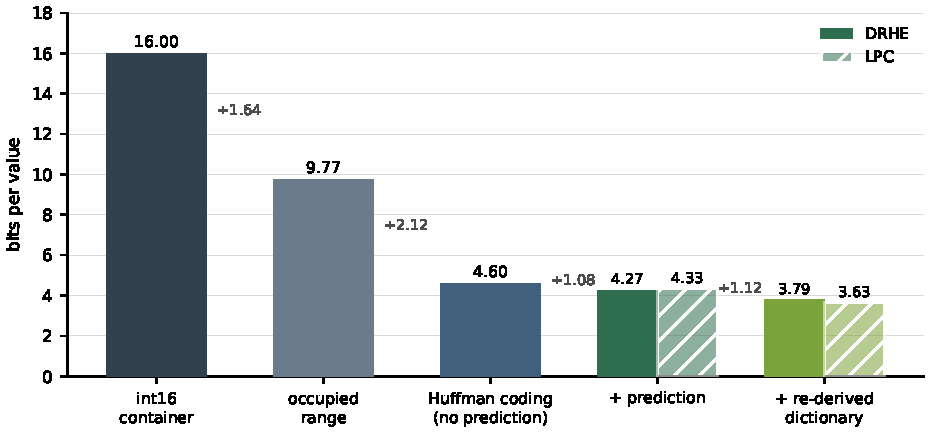
\includegraphics[width=0.85\textwidth]{fig_bits.pdf}
\caption[Where the bits go]{Bits per value through the compressor, 50 frames,
four receive channels. Most of the reduction comes from the unused top of the
16-bit container and from the sparsity of the data, before any prediction.
Factors are for DRHE; LPC is shown hatched.}
\label{fig:bits}
\end{figure}

Two consequences follow.

\paragraph{The ratios are partly a property of the capture.} A sensor whose
data filled the 16-bit container would have no unused top bits to remove. Its
extra bits would instead hold finer detail of the receiver noise, which a
lossless coder must keep, and the quantisation study of Section~\ref{sec:quant}
shows what that does: scaled to fill the container, the same frame compresses
by only \num{1.2}. Ratios measured on different sensors are therefore not
directly comparable unless their gain staging is. A no-prediction
baseline should be reported alongside any radar compression ratio; it costs a
few lines of MATLAB and separates the algorithm from the sensor.

\paragraph{The unused bits are a design choice.} The same unused bits are why
FX16 loses \SI{3.77}{\percent} of targets: filling the container removes that
loss and, with it, most of the compression (Section~\ref{sec:quant}). How many
bits of the noise floor are worth transmitting is a decision for the radar
system designer; a lossless compressor does not change that trade, it only
makes whatever choice is made cheaper to carry.

\section{How far the dictionary and the lag generalise}
\label{sec:generalise}

The re-derived dictionaries were trained on five frames of one recording and
tested on 45 later frames of the same recording, where they hold within
\SI{1}{\percent}. That shows they do not over-fit the training frames; it does
not show they transfer to other scenes, sensors or gain settings. Because a
dictionary is a sixteen-entry table, a production design could hold several and
choose per frame, or update one slowly from the statistics of past frames,
without changing anything else in the hardware.

The prediction lag is specific in its value and general in its principle. It
is $\nTx = 12$ because this radar rotates twelve transmitters in a fixed
order; a radar that changed its MIMO schedule would need the lag reloaded, and
one using Doppler- or code-division multiplexing has no interleaved ramp axis.
The principle --- a slow-time predictor must predict from the same antenna ---
applies to any slow-time coder carried over from a single-transmitter design to
a time-multiplexed one, and the check is cheap: if the predictor does not beat
the no-prediction baseline, it is predicting along the wrong axis.

\section{Hardware cost against the baseline design}
\label{sec:hwvskiem}

Table~\ref{tab:hwvskiem} sets the hardware beside Kiem's. The designs differ in
board, data and system, so the comparison is of methods rather than of chips.

\begin{table}[htbp]
\centering
\caption[Hardware against the baseline]{This thesis's hardware against Kiem's
\cite{kiem2025}. Different boards (Zynq \texttt{XCZU3CG} against Kintex
\texttt{XCKU5P}, both UltraScale+), radars and data. Core resources are the
compressor alone; BRAM in 36\,Kb blocks.}
\label{tab:hwvskiem}
\footnotesize
\setlength{\tabcolsep}{4pt}
\begin{tabular}{@{}lrrr@{}}
\toprule
& Kiem & This work: DRHE & This work: LPC\\
\midrule
Lossless CR in hardware      & \num{3.17} & \num{3.75} & \num{3.70}\\
CR, re-derived dictionary (C-sim) & --- & \num{4.22} & \num{4.40}\\
Hardware checked against simulation & no & byte-identical & byte-identical\\
Decompressor                 & none & PC; on chip\textsuperscript{a} & PC; on chip\textsuperscript{a}\\
Throughput                   & \SI{11.92}{Gibit/s} (theor.) & \SI{4.77}{Gibit/s} (meas.) & \SI{0.90}{Gibit/s} (meas.)\\
End-to-end latency           & \SI{79.4}{\micro\second}\textsuperscript{b} & \SI{13.1}{\micro\second} & \SI{3006}{\micro\second}\\
Compressor LUT / FF          & \num{45892} / \num{9243} & \num{35444} / \num{23528} & \num{33738} / \num{20165}\\
Compressor BRAM / DSP        & 10 / 44 & 40 / 132 & 98 / 158\\
Arithmetic                   & fixed point, $\mathrm{II} = 1$ & floating point, $\mathrm{II} = 2$ & fixed point, $\mathrm{II} = 1$\\
\bottomrule
\multicolumn{4}{@{}l}{\footnotesize\textsuperscript{a}built and verified in C-simulation; board run pending.\quad \textsuperscript{b}includes his FFT core.}
\end{tabular}
\end{table}

Three points need care in reading it.

\paragraph{Throughput units.} Kiem's \SI{11.92}{Gibit/s} is $128$ bits per clock
at \SI{100}{\mega\hertz} expressed in binary units:
$11.92 \times 2^{30} / 10^8 = 128.0$ bits per cycle, the full width of the input
stream at $\mathrm{II} = 1$. It is a theoretical rate. The comparable figure
for DRHE here is \SI{6.4}{Gbit/s} at $\mathrm{II} = 2$; measured on the board,
including DMA and per-ramp pipeline fill, it achieves \SI{5.12}{Gbit/s}
(\SI{4.77}{Gibit/s}).

\paragraph{Latency.} Kiem's \SI{79.4}{\micro\second} runs from the last DMA
read to the last DMA write of a system that includes an FFT core in front of
the compressor; the \SI{13.1}{\micro\second} here uses the same definition
without an FFT. The two are the same kind of quantity but not the same
pipeline.

\paragraph{Where the logic goes.} DRHE here uses fewer LUTs than Kiem's
compressor but three times the DSPs and four times the block RAM. To account
for the difference, the rebuilt replica and ladder of variants of
Section~\ref{sec:repbaseline} were used. Against that replica every difference
has one identified cause: the floating-point
datapath, above all the arctangent units, accounts for most of the logic, the
DSPs and the pipeline depth (58 stages against 12); 32-bit floating-point state
words double the block RAM; the per-transmitter state of
Section~\ref{sec:predaxis} doubles it again; and $\mathrm{II} = 2$ comes from
one extra write per cycle to reset the state (Section~\ref{sec:drheimpl}).
Changing only the arithmetic to Kiem's fixed-point types compresses ColoRadar to
within \SI{0.07}{\percent} of the floating-point design. The floating-point
datapath, which Kiem had suggested investigating, is the most expensive design
decision in this thesis and buys almost nothing; fixed point is the first
improvement to make.

\section{Comparison with the baseline's results}
\label{sec:vskiem}

Kiem reports a ratio of \num{3.25} in simulation for DRHE; this thesis measures
\num{3.75} with the same dictionary. The two numbers come from different
sensors and different data. The rebuilt simulation of
Section~\ref{sec:repbaseline} connects them, with three results.

\begin{itemize}
\item \textbf{His DRHE results are reproduced.} At a noise level of
$-87.9$\,dBFS, where the FX16 noise is \num{4.63} LSB, the rebuilt chain gives
\num{3.25} with run-length coding and \num{3.24} without, his two figures. His
dictionary is optimal for residuals with a standard deviation of 6 to 8 LSB, and
his ratio is what a matched dictionary gives on residuals of that size. At the
noise level stated for his synthetic scene the same chain gives only
\num{2.28}, which confirms that his published ratios come from his recordings,
not from that scene.

\item \textbf{The algorithm is the same.} Running the rebuilt chain and this
thesis's DRHE side by side on the same input gives bit-identical output: the
DRHE here is Kiem's specification exactly, apart from the prediction lag, which
on his single-transmitter radar is 1 because $\nTx = 1$.

\item \textbf{Two methods called LPC.} Kiem excluded LPC-Huffman as less
promising than DRHE without running it. Run on his scene, that method ---
fast-time prediction of raw ADC samples --- compresses by only \num{1.32} to
\num{1.54}, largely because it codes ADC noise that the FX16 step discards. His
judgement of that method stands. The slow-time LPC of this thesis is a
different design, and it compresses as well as DRHE.
\end{itemize}

\noindent
Taken together, the comparison says that Kiem's DRHE carries over to a
twelve-transmitter cascade unchanged except for the prediction lag; that with
the lag set correctly and the dictionary matched to the data it compresses
public cascade data by \num{4.2} (a different sensor and scene from his
\num{3.2}, so not a like-for-like comparison); and that it can be verified bit
for bit on hardware with a decoder, which his system could not.

\section{Threats to validity}
\label{sec:threats}

\begin{itemize}
\item \textbf{The ratios are capture-specific.} Much of the ratio comes from an
under-filled container (Section~\ref{sec:ratiomeaning}), a property of this
recording's gain staging.

\item \textbf{One recording.} All results use 50 consecutive frames of one
ColoRadar sequence. Scenes with more or faster targets would give larger
prediction errors and lower ratios, and the re-derived dictionaries were
trained and tested on the same recording.

\item \textbf{The detection metrics measure the quantisation step.} The three
lossless schemes share FX16's detection metrics by construction. The detection
chain is also simpler than a production one: its Doppler FFT runs across all 192
ramps in recorded order, it has no angle FFT, detections are matched cell by
cell with no positional tolerance, and the threshold is not swept. The
absolute rates of the lossy schemes should therefore be read as relative.

\item \textbf{BAQ is a block-floating-point stand-in.} A better-tuned,
statistics-driven BAQ could lose fewer detections at the same ratio; it would
still be lossy.

\item \textbf{Channel count differs between stages.} Stage~1 uses all 16
receive channels; Stage~2 and the hardware use four. The two stages' ratios are
close (\num{3.75} and \num{3.751} for DRHE) but not identical by construction.

\item \textbf{Some board measurements are outstanding.} The board run with the
original dictionary is complete. The re-derived-dictionary bitstreams and the
on-chip decompressors are built, meet timing and are verified in simulation,
but their board runs, and hence the decompressors' measured time and latency,
are \pending{to be added}. Power was not measured.

\item \textbf{Co-simulation covers one frame.} The 50-frame results are from
C-simulation and the board, which exercise identical logic; the cycle-accurate
RTL simulation was run on one frame.

\item \textbf{The baseline was rebuilt from its description.} Kiem's source code
and recordings are not public. The replica of his hardware and his simulation
follow every type, function and parameter his thesis states; the parts it does
not state are this thesis's reading of it.
\end{itemize}
